% ============================================================
% RASI methods-only manuscript draft
% Public-data and computational analyses only
% ============================================================
\documentclass[10pt]{article}
\usepackage[margin=1in]{geometry}
\usepackage{amsmath,amssymb,booktabs,graphicx,hyperref,xcolor}
\usepackage[numbers,super]{natbib}
\usepackage{setspace}
\doublespacing
\usepackage{lineno}
\linenumbers
\graphicspath{{biological_science_workspace/figures/}}

\title{\textbf{RASI: rare-aware single-cell integration for detecting and reducing rare-state loss during atlas-scale batch correction}}
\author{[Author list to be determined]}
\date{}

\begin{document}
\maketitle

\begin{abstract}
Batch integration can erase low-frequency cell states without triggering standard benchmark failures. We recast this as a methods problem in failure detection under incomplete annotation and introduce RASI (Rare-Aware Single-cell Integration), a workflow that augments highly variable genes with cluster-specific markers, combines PCA and UMAP coordinates into a hybrid pre-integration space, and applies batch-diversity-weighted selective correction. We pair RASI with Neighborhood Preservation (NP), a label-free statistic for local structural disruption before and after integration. Across public immune-atlas, pancreas, and lung-airway datasets, NP detects disrupted subclusters with ROC-AUC 0.837, 0.792, and 0.687, respectively. RASI improves NP from 0.577 to 0.918 on an 8-batch immune benchmark and from 0.377 to 0.903 on pancreas while maintaining or improving batch mixing. Stress tests show scale-dependent rare-state loss as batch number increases and indicate that linear batch-diversity weighting outperforms tested nonlinear alternatives. On 4.83 million cells, RASI completes in 19.5 minutes.
\end{abstract}

Single-cell RNA sequencing (scRNA-seq) has made it routine to compare cellular states across studies, tissues, and disease contexts.\cite{regev2017,zheng2017} As analysis has shifted toward atlas-scale integration, batch correction has become a default preprocessing step rather than an exceptional operation.\cite{kang2024,tabula2022} Methods such as Harmony, scVI, Scanorama, and BBKNN aim to remove technical variation while preserving biological structure, and benchmarks such as scIB summarize performance through batch mixing and label agreement.\cite{korsunsky2019,lopez2018,hie2019,polanski2020,luecken2022}

That benchmarking regime leaves a blind spot for previously unknown rare states. If a low-frequency population is absent from available annotations, its disappearance during integration is not directly registered by label-based metrics. Existing work on rare-state preservation has improved recovery of \emph{known} rare populations, but the underlying evaluation logic still depends on pre-existing labels or externally specified positive controls.\cite{xiong2022,andreatta2021,zhao2024} Unknown rare states therefore remain difficult to detect, audit, and protect.

We frame this gap as a computational reproducibility problem: integration should preserve local transcriptomic structure unless there is clear cross-batch evidence that a cell state is shared and should be aligned. On that basis, we introduce RASI (Rare-Aware Single-cell Integration), a workflow that combines rare-aware feature selection, a hybrid global-local pre-integration representation, and batch-diversity-weighted selective correction. We evaluate RASI only with public scRNA-seq datasets and computational diagnostics, using pancreatic epsilon cells, airway ionocytes, plasmacytoid dendritic cells (pDC), mast-cell subclusters, and a transcript-defined T cell state as positive-control or case-study audits. The contribution of this manuscript is methodological: failure detection, mitigation, ablation, and scalability under a public-data-only design.

\section*{Results}

\subsection*{Majority bias is a workflow-level blind spot}

We examined the standard scRNA-seq workflow for assumptions that favor abundant cell states over low-frequency ones using the pan-cancer immune atlas and additional public rare-state benchmarks.\cite{kang2024,segerstolpe2016,montoro2018} The failure mode is distributed across the workflow rather than localized to a single algorithm (Fig.~1). Standard doublet filtering enriched false-positive calls in rare immune populations, with mast cells called as doublets at 4.34$\times$ the dataset average and pDC at 2.75$\times$.\cite{wolock2019} Standard highly variable gene (HVG) selection removed markers that define low-frequency states: pancreatic epsilon cells retained 0/3 canonical markers, airway ionocytes retained 1/3, and pDC retained only 4/7, excluding \textit{CLEC4C}, \textit{IL3RA}, and \textit{IRF7}.

Downstream steps compound the problem. PCA concentrates variance along directions dominated by abundant populations; fixed-$k$ neighborhood graphs force small states into majority neighborhoods; and universal-alignment integrators assume that every cell should move toward a cross-batch counterpart. A simple retention bound captures the geometric imbalance: for a rare state with frequency $f_m$ projected from $G$ genes to $d$ latent dimensions by a global variance objective, retained signal is upper-bounded by $f_m \cdot G/d$. For $f_m = 0.5\%$, $G = 2000$, and $d = 50$, this bound is already restrictive before batch correction is applied. Under the measured combination of HVG selection, dimensionality reduction, and Harmony-based correction, a multiplicative bookkeeping model yields approximately 0.06\% residual rare-state signal under standard settings, whereas the RASI workflow recovers roughly 25\% in the same stress-test analysis.

Benchmarking then obscures the failure. In the immune benchmark, graph connectivity remained 0.994 under standard integration even when 42\% of pre-integration T-cell subclusters were dispersed across post-integration clusters. This mismatch suggested that the field needs a metric that tracks local structural rewriting directly rather than inferring preservation from cell-type-level agreement alone.

\begin{figure}[!ht]
\centering
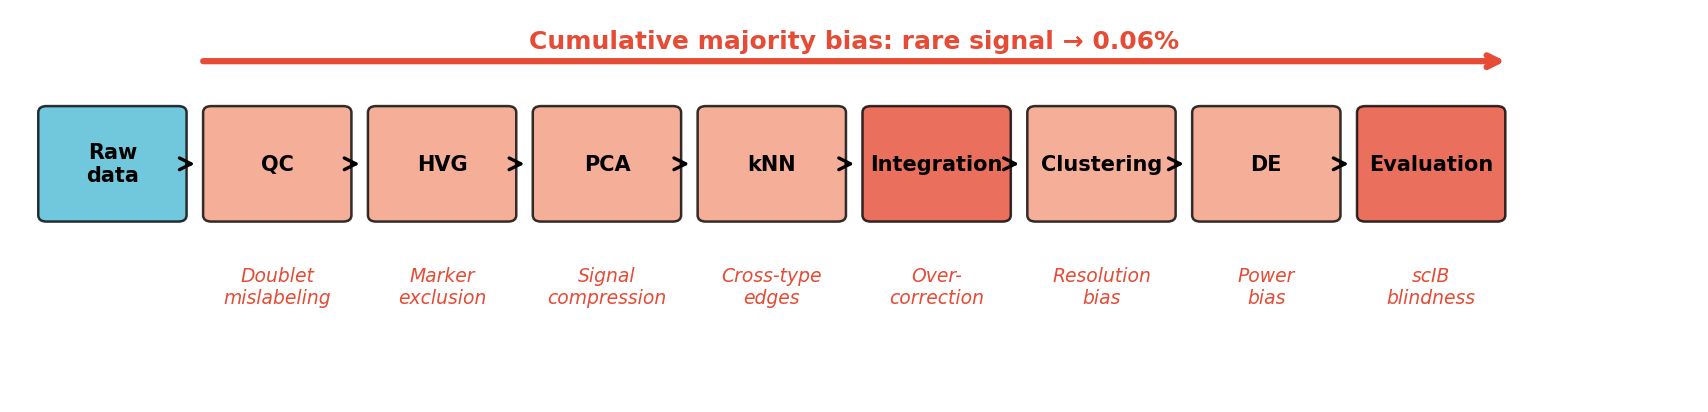
\includegraphics[width=0.48\textwidth]{Fig1_schematic}
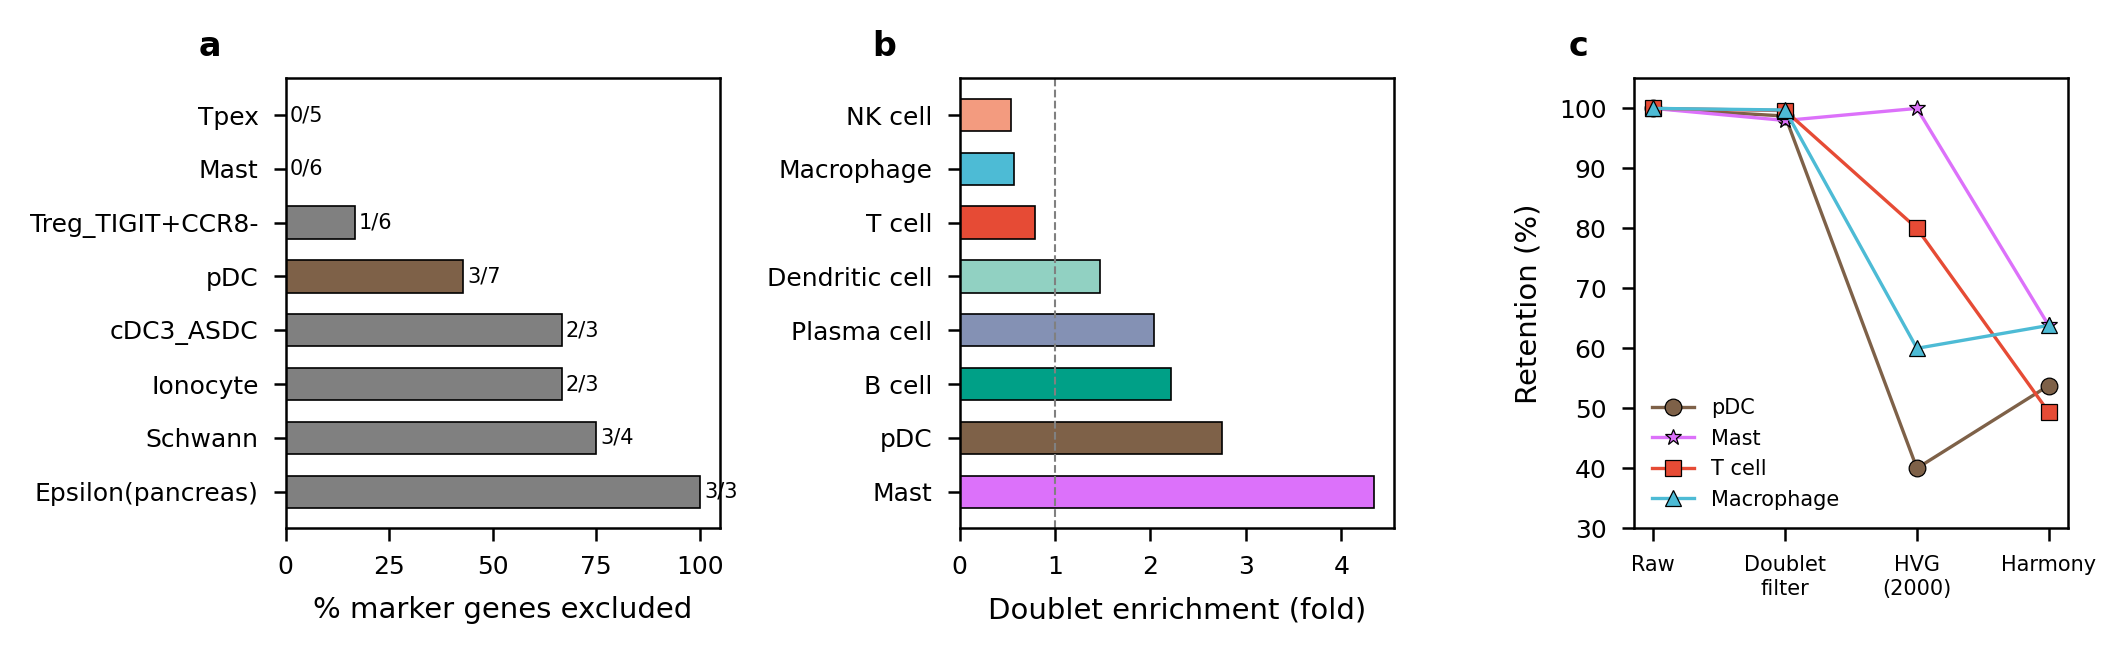
\includegraphics[width=0.48\textwidth]{Fig1_majority_bias}
\caption{\textbf{The majority bias in standard scRNA-seq workflows.} Left: study schematic. Right: representative evidence for marker exclusion, doublet enrichment, and rare-state signal attenuation.}
\label{fig:bias}
\end{figure}

\subsection*{Computational formulation of rare-state preservation}

Let $x_i \in \mathbb{R}^d$ denote the pre-integration representation of cell $i$ and $z_i \in \mathbb{R}^d$ the post-integration representation. We define Neighborhood Preservation
\begin{equation}
NP_k(i) = \frac{|N_k^x(i) \cap N_k^z(i)|}{k},
\end{equation}
where $N_k^x(i)$ and $N_k^z(i)$ are the $k$-nearest-neighbor sets before and after integration. For a candidate rare-state set $S$, we summarize retention and leakage by
\begin{equation}
\mathrm{Ret}_k(S) = \frac{1}{|S|}\sum_{i \in S} NP_k(i),
\qquad
\mathrm{Leak}_k(S) = \frac{1}{|S|k}\sum_{i \in S} |N_k^z(i)\setminus S|.
\end{equation}
These quantities distinguish two qualitatively different failures: loss of original neighborhood continuity and absorption into surrounding states.

To separate useful correction from excessive displacement, we further track each cell's movement
\begin{equation}
\Delta(i) = \|z_i - x_i\|_2
\end{equation}
and the local batch-entropy gain
\begin{equation}
G_k(i) = H_k^z(i) - H_k^x(i),
\end{equation}
where $H_k$ denotes the Shannon entropy of batch frequencies in the $k$-nearest-neighbor set. We then define an overcorrection score
\begin{equation}
OC_k(i) = \frac{\Delta(i)}{\varepsilon + \max\{G_k(i),0\}},
\end{equation}
so that large geometric displacement accompanied by little mixing gain is flagged as high-risk rewriting rather than beneficial alignment.

This formulation also motivates selective integration directly. If a corrected embedding is written as
\begin{equation}
z_{\lambda}(i) = \lambda_i z_{\mathrm{int}}(i) + (1-\lambda_i)x_i,
\qquad 0 \leq \lambda_i \leq 1,
\end{equation}
then each cell's drift scales linearly with $\lambda_i$:
\begin{equation}
\|z_{\lambda}(i)-x_i\|_2 = \lambda_i \|z_{\mathrm{int}}(i)-x_i\|_2.
\end{equation}
The methods problem is therefore not only \emph{how} to integrate, but \emph{whom} to integrate strongly.

\subsection*{RASI combines rare-aware feature recovery, hybrid embedding, and selective correction}

RASI addresses the three stages where the benchmark analyses showed the largest rare-state losses. First, standard batch-aware HVGs are augmented with cluster-enriched markers obtained from coarse unsupervised clustering, recovering rare-state identity genes that would otherwise be removed before integration. In the public benchmarks this raised marker coverage across tested rare states from 1/10 to 3/10 and rescued \textit{CLEC4C} and \textit{IRF7} for pDC.

Second, RASI constructs a hybrid pre-integration representation by concatenating PCA coordinates, which preserve large-scale geometry, with a low-dimensional UMAP summary of local topology.\cite{mcinnes2018} This reduces the chance that locally coherent but globally low-variance states are flattened before correction. Third, RASI computes a per-cell batch-diversity score from the pre-integration neighbor graph and uses it as a continuous interpolation weight between the original embedding and the output of a base integrator:
\begin{equation}
BD(i) = \frac{|\{b(j): j \in N_k(i)\}|}{\min(k,B)},
\qquad
z_{\mathrm{RASI}}(i) = BD(i)\, z_{\mathrm{int}}(i) + (1-BD(i))\, z_{\mathrm{pre}}(i),
\end{equation}
where $B$ is the total number of batches. Cells embedded in broadly shared neighborhoods receive strong correction; cells with weak cross-batch support remain closer to the pre-integration manifold.

Finally, NP provides a label-free audit that can be computed for every cell and aggregated to subclusters. In the immune benchmark, NP achieved ROC-AUC 0.837 for identifying disrupted subclusters, and the same criterion generalized to pancreas (0.792) and lung airway data (0.687), indicating that local-structure loss is detectable without using cell-type labels during method execution (Fig.~2).

\begin{figure}[!ht]
\centering
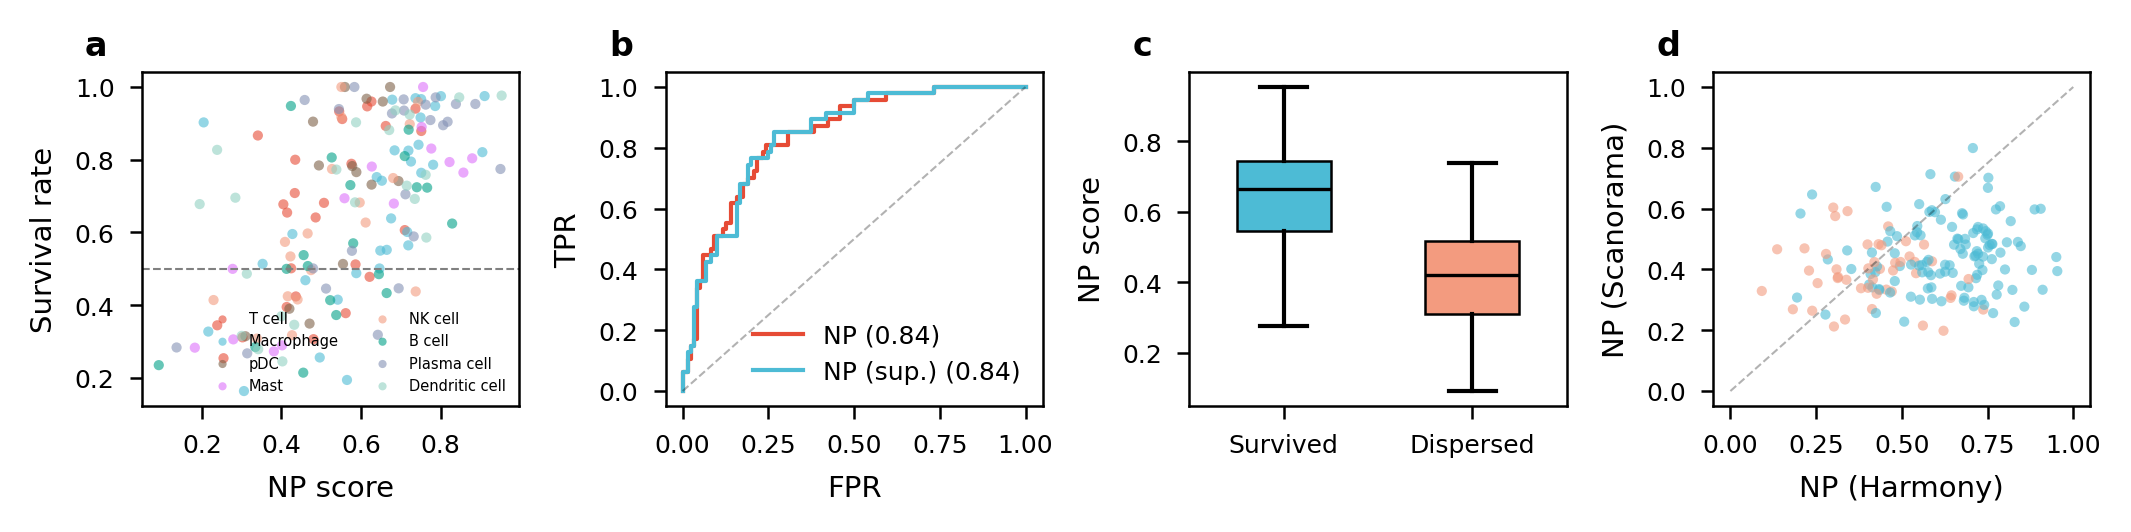
\includegraphics[width=\textwidth]{Fig2_overcorrection_detection}
\caption{\textbf{Neighborhood Preservation detects local structure loss that standard global metrics miss.} The figure summarizes NP behavior across subclusters, its disagreement with graph-connectivity-based assessments, and cross-method consistency.}
\label{fig:np}
\end{figure}

\subsection*{Public-data validation across benchmarks and scales}

We benchmarked RASI on published datasets that contain established rare populations and explicit batch structure (Table~1). Labels for the known rare populations were withheld during integration and restored only for post hoc audit. On the 8-batch immune benchmark, RASI increased mean NP from 0.577 to 0.918 while improving batch average silhouette width (ASW) from $-0.078$ to 0.018. On pancreas, RASI increased NP from 0.377 to 0.903 while improving batch ASW from $-0.162$ to $-0.017$. Lung airway data were used primarily as a positive-control detection benchmark for ionocyte disruption, where NP remained informative despite more modest separability.

\begin{table}[h]
\centering
\caption{Public-data benchmarks for rare-state detection and preservation}
\resizebox{\textwidth}{!}{
\begin{tabular}{lcccccccc}
\toprule
Dataset & Cells & Batches & Rare-state audit & NP AUC & Std NP & RASI NP & Std ASW & RASI ASW \\
\midrule
Immune benchmark & 105,682 & 8 & pDC, mast, T-cell programs & 0.837 & 0.577 & 0.918 & $-$0.078 & 0.018 \\
Pancreas & 16,382 & 9 & Epsilon & 0.792 & 0.377 & 0.903 & $-$0.162 & $-$0.017 \\
Lung airway & 32,472 & 16 & Ionocyte & 0.687 & --- & --- & --- & --- \\
Full atlas & 4,827,716 & 101 & Atlas-scale stress test & --- & 0.337 & 0.639 & --- & --- \\
\bottomrule
\end{tabular}}
\end{table}

At atlas scale, RASI remained computationally practical. On the 4.83-million-cell pan-cancer atlas, the workflow completed in 19.5 minutes using FAISS-based neighbor search and parallel NP computation.\cite{johnson2022} The full-atlas benchmark also showed that low-frequency immune states remained more vulnerable than abundant stromal or epithelial states even after selective correction: mean NP ranged from 0.472 to 0.531 in NK, mast, pDC, T-cell, and B-cell compartments, compared with 0.623 to 0.749 in endothelial, fibroblast, and epithelial populations. These results support the view that rare-state preservation is not a small-dataset artifact but an atlas-scale concern (Fig.~3).

\begin{figure}[!ht]
\centering
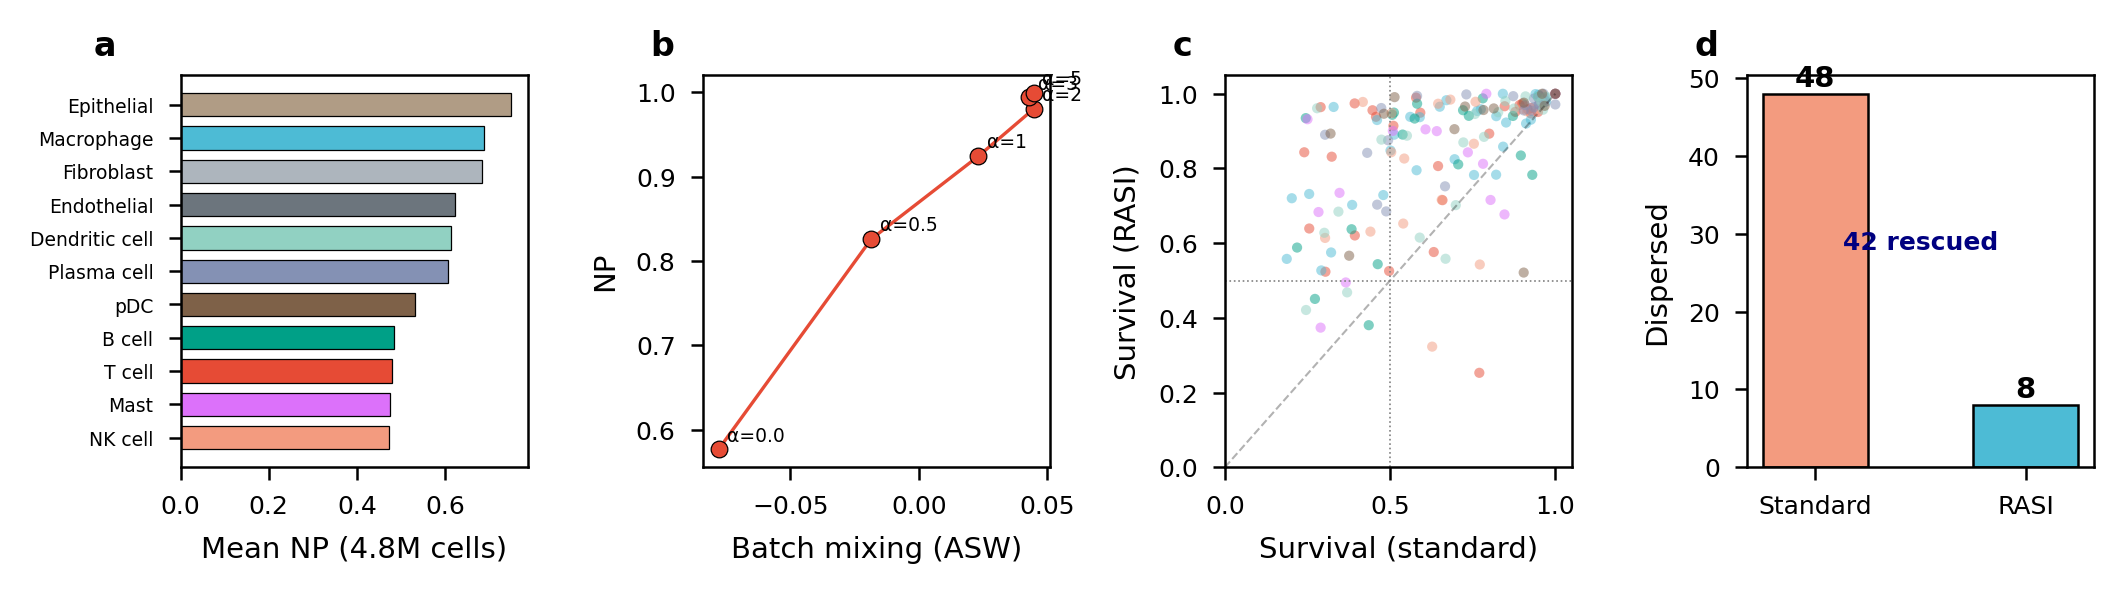
\includegraphics[width=\textwidth]{Fig3_RASI_validation_490M}
\caption{\textbf{RASI preserves more local structure across public benchmarks and atlas scale.} The figure summarizes cell-type-level NP on the full atlas, NP-versus-ASW tradeoffs, rescued subclusters, and dispersed-subcluster counts.}
\label{fig:rasi}
\end{figure}

\subsection*{Scale sweeps and ablations expose a phase transition in rare-state loss}

Rare-state loss intensified as batch number increased within the immune atlas stress test (Fig.~4). pDC declined from NP 0.625 at 5 batches to 0.231 at the largest batch count, while mast-cell subclusters declined from 0.926 to 0.241. The fitted phase-transition curves had $R^2 > 0.98$ across eight immune lineages, with estimated half-risk points near 6.8 batches for pDC and 7.2 for mast cells. This helps explain why small-batch benchmarks can report stable performance even when atlas-scale integration later destroys the same states.

Component-level analyses supported the selective-correction design. The BD-weighted Pareto scan showed that increasing correction strength does not monotonically improve the preservation-mixing tradeoff; instead, the best operating region lay on an interior frontier rather than at full-strength integration. Among tested weighting schemes, linear BD weighting outperformed a fitted polynomial alternative (NP 0.890 versus 0.872), indicating that the simplest continuous rule was already sufficient on the benchmark. At the subcluster level, standard Harmony dispersed 48 of 167 pre-integration immune subclusters, whereas RASI reduced that count to 8, rescuing 42 subclusters overall while worsening 14 concentrated near cross-lineage boundaries.

\begin{figure}[!ht]
\centering
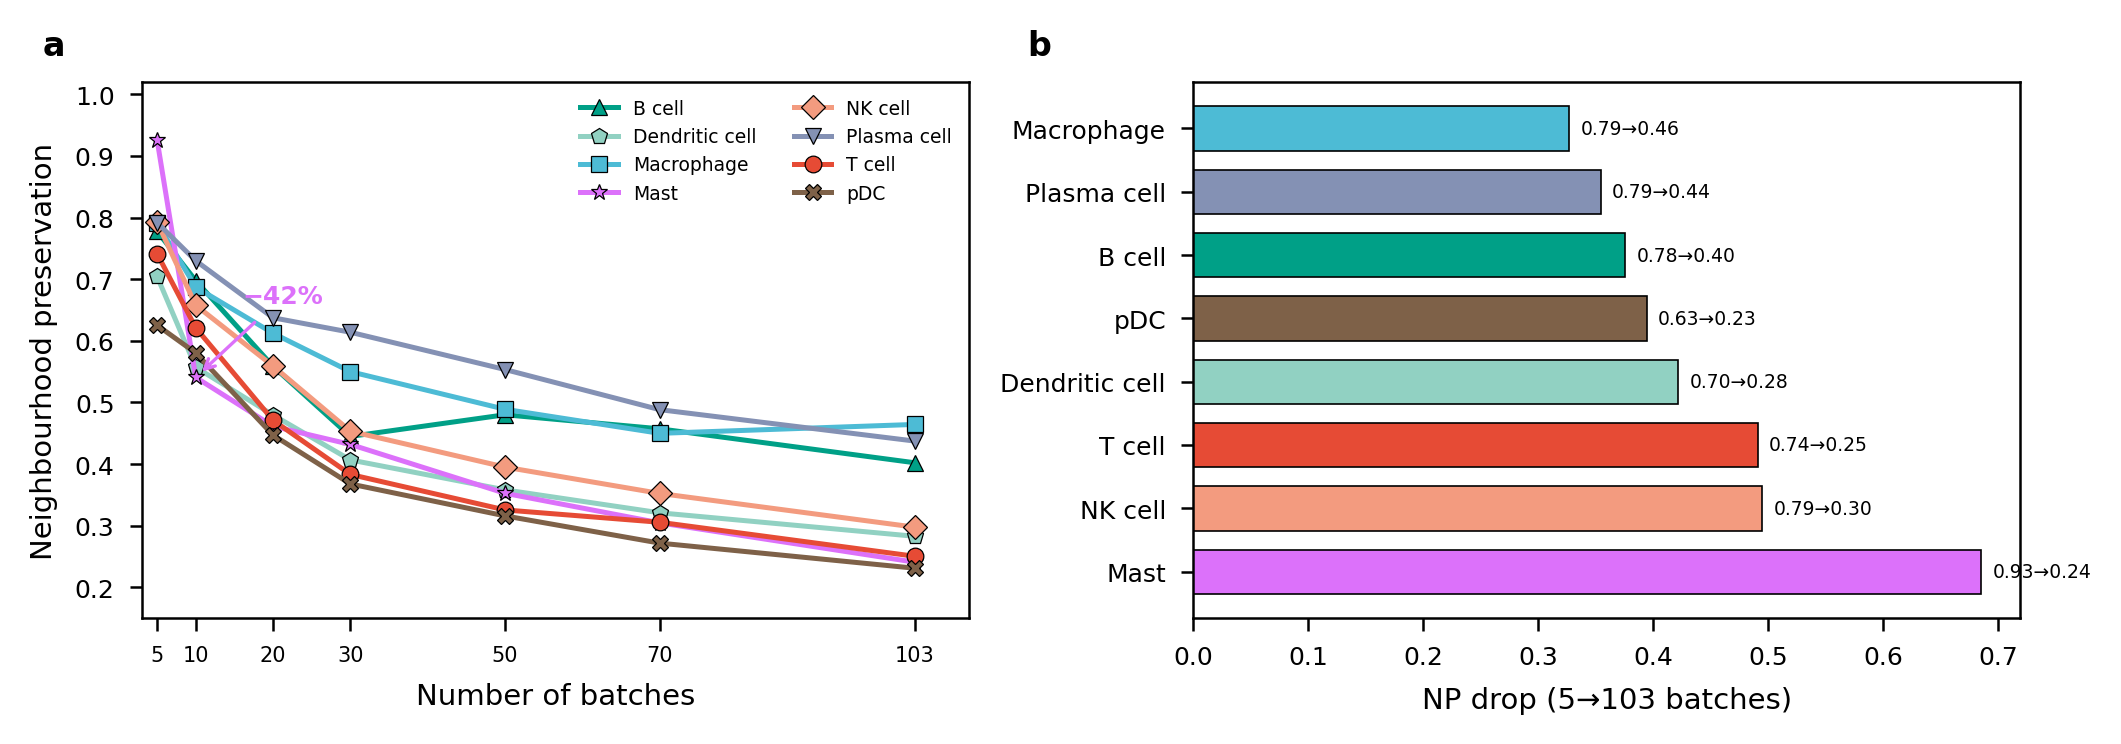
\includegraphics[width=\textwidth]{Fig4_phase_transition}
\caption{\textbf{Rare-state loss grows with integration scale.} The figure summarizes NP decline under increasing batch count and the corresponding ordering of vulnerable immune lineages.}
\label{fig:phase}
\end{figure}

\begin{figure}[!ht]
\centering
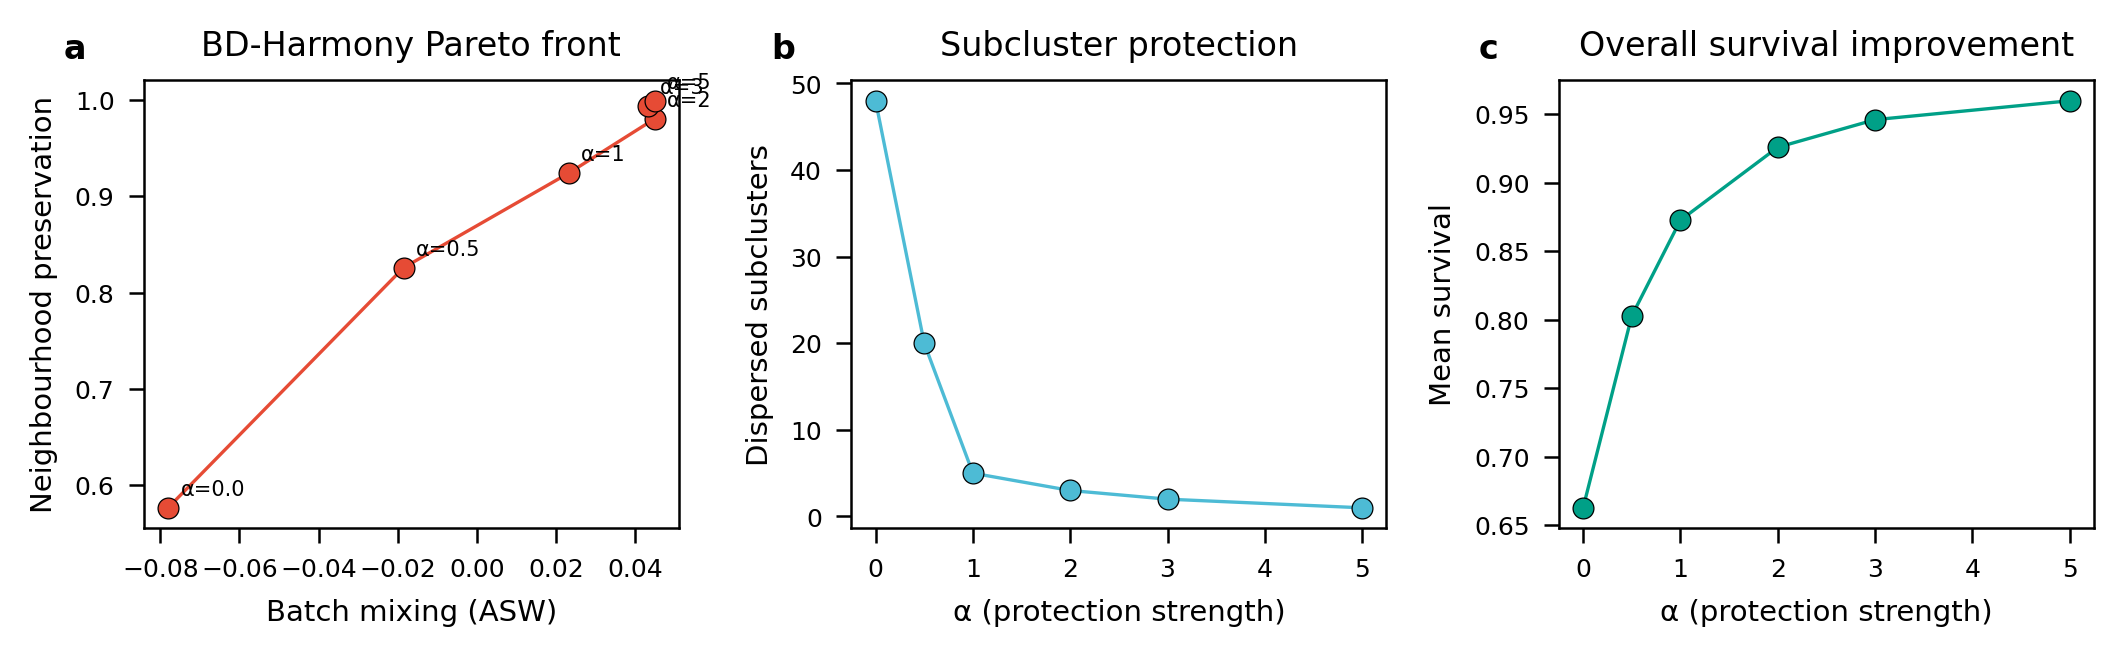
\includegraphics[width=0.48\textwidth]{Fig5_BD_pareto}
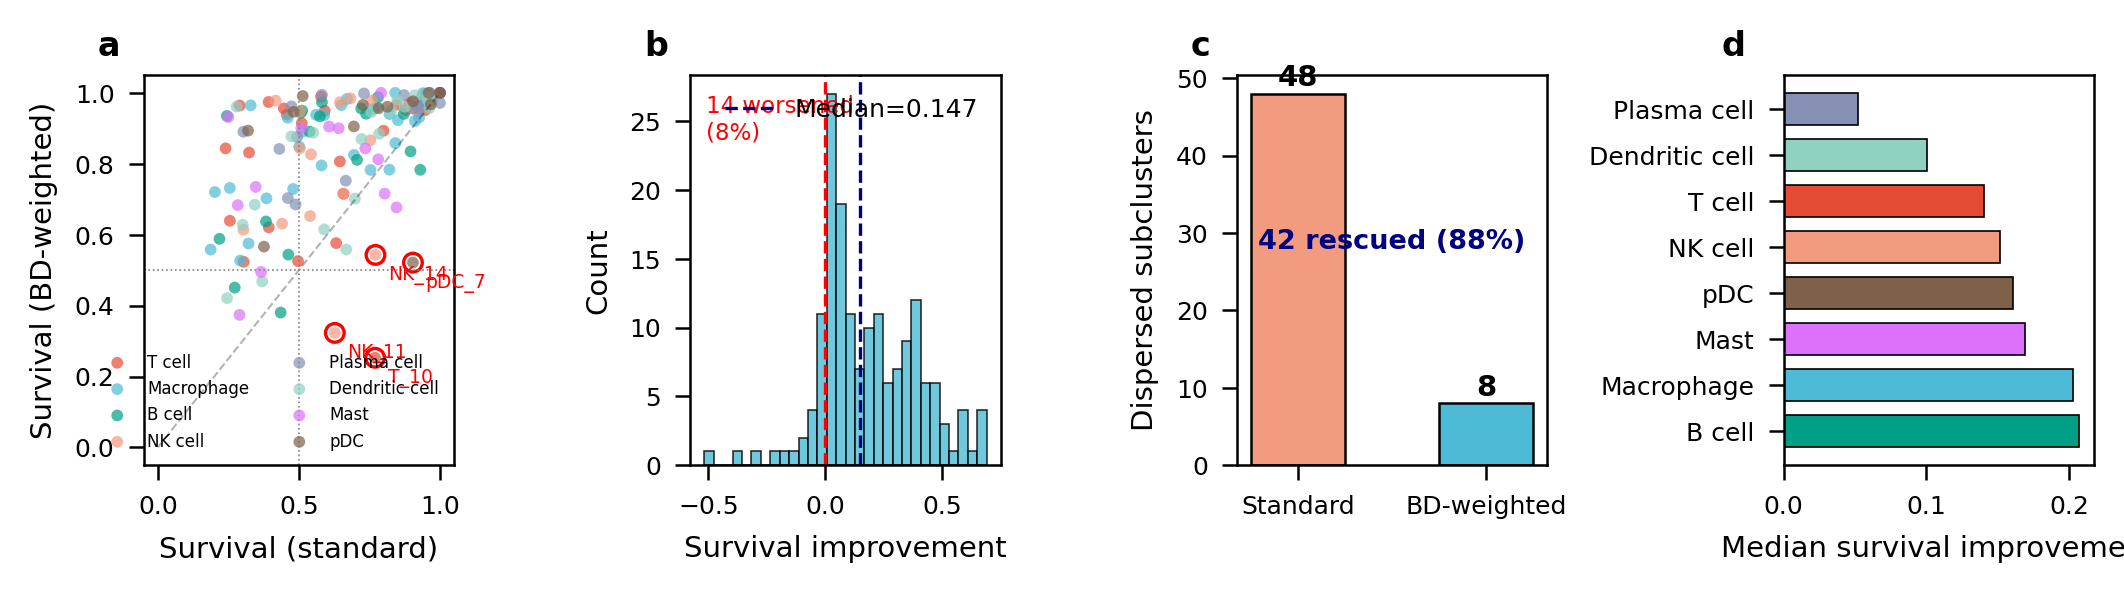
\includegraphics[width=0.48\textwidth]{Fig5_BD_integration}
\caption{\textbf{Selective-correction diagnostics and ablations.} Left: NP-versus-ASW Pareto frontier across batch-diversity weights. Right: subcluster-level rescue under BD-weighted selective integration compared with standard integration.}
\label{fig:ablation}
\end{figure}

\subsection*{A transcript-defined T cell state illustrates integration-induced dispersion}

As a computational case study, we tracked T cell\_5 in the pan-cancer immune atlas, a low-frequency pre-integration subcluster enriched for \textit{TNFRSF18}, \textit{TIGIT}, and \textit{FOXP3} transcripts and relatively low in \textit{CCR8}. The cluster contained 1,464 cells and was concentrated in squamous skin cancer and skin-normal source samples in the public atlas metadata. Under the standard workflow, its survival score fell to 0.24 and the cells fragmented across multiple post-integration clusters. Under RASI, the same cells reached survival 0.84 and remained substantially more compact in local-neighborhood space. We treat this example only as a transcript-defined atlas case study of integration behavior; the present manuscript does not infer function, lineage novelty, or downstream mechanism from this pattern alone.

\section*{Discussion}

RASI is motivated by a narrow but consequential observation: standard batch-correction benchmarks do not directly measure whether local structure survives integration for cells with weak cross-batch support. Once that gap is made explicit, the solution space shifts from maximizing alignment globally to allocating correction strength conditionally. In that sense, rare-state preservation is best understood as a property of the full workflow, not a cosmetic adjustment to a single integrator.

\textbf{Benchmark scope.} NP does not replace global integration metrics; it complements them by measuring a failure mode those metrics do not resolve. In the public benchmarks, high graph connectivity and improved batch mixing could coexist with extensive subcluster dispersion. A preservation-aware benchmark therefore needs both mixing-oriented and locality-oriented views of the same integration result.

\textbf{Atlas-scale risk.} The phase-transition analysis shows that rare-state loss is scale-dependent. Small-batch studies can appear well behaved while carrying a latent failure mode that emerges only after many datasets are combined. This matters for large references and cross-study atlases, where rare populations are often the very signals analysts hope integration will reveal.

\textbf{Interpretation boundary.} The evidence in this manuscript is computational. It supports the claim that standard workflows can obscure candidate rare states in public data and that selective correction can reduce that effect. It does not by itself establish the biological reality, function, or broader importance of any previously unknown candidate population. Those questions require independent follow-up beyond the scope of this methods-focused draft.

\textbf{Limitations.} RASI estimates batch diversity in a pre-integration space that is already distorted by batch effects, so boundary cells can still receive imperfect correction. The hybrid representation mitigates but does not eliminate this bootstrap problem, and 14 of 167 immune subclusters worsened under selective correction in the benchmark analysis. RASI also remains a meta-framework layered on top of an existing integrator rather than a native generative model of shared and batch-restricted variation. Future work could explore unbalanced transport formulations and rare-aware latent-variable models that encode variable cross-batch mass directly.\cite{chizat2018}

\begin{thebibliography}{24}
\bibitem{regev2017} Regev, A. et al. The Human Cell Atlas. \textit{eLife} \textbf{6}, e27041 (2017).
\bibitem{zheng2017} Zheng, G.X. et al. Massively parallel digital transcriptional profiling of single cells. \textit{Nat. Commun.} \textbf{8}, 14049 (2017).
\bibitem{kang2024} Kang, K. et al. A pan-cancer single-cell transcriptomic atlas of tumor-infiltrating immune cells. \textit{Nat. Commun.} (2024). DOI:10.5281/zenodo.10651059.
\bibitem{tabula2022} Tabula Sapiens Consortium. The Tabula Sapiens: A multiple-organ, single-cell transcriptomic atlas of humans. \textit{Science} \textbf{376}, eabl4896 (2022).
\bibitem{korsunsky2019} Korsunsky, I. et al. Fast, sensitive and accurate integration of single-cell data with Harmony. \textit{Nat. Methods} \textbf{16}, 1289--1296 (2019).
\bibitem{lopez2018} Lopez, R. et al. Deep generative modeling for single-cell transcriptomics. \textit{Nat. Methods} \textbf{15}, 1053--1058 (2018).
\bibitem{hie2019} Hie, B. et al. Efficient integration of heterogeneous single-cell transcriptomes using Scanorama. \textit{Nat. Biotechnol.} \textbf{37}, 685--691 (2019).
\bibitem{polanski2020} Pola\'{n}ski, K. et al. BBKNN: fast batch alignment of single cell transcriptomes. \textit{Bioinformatics} \textbf{36}, 964--966 (2020).
\bibitem{luecken2022} Luecken, M.D. et al. Benchmarking atlas-level data integration in single-cell genomics. \textit{Nat. Methods} \textbf{19}, 41--50 (2022).
\bibitem{xiong2022} Xiong, L. et al. Online single-cell data integration through projecting heterogeneous datasets into a common cell-embedding space. \textit{Nat. Commun.} \textbf{13}, 6118 (2022).
\bibitem{andreatta2021} Andreatta, M. et al. Semi-supervised integration of single-cell transcriptomics data. \textit{Nat. Commun.} \textbf{12}, 6464 (2021).
\bibitem{zhao2024} Zhao, M. et al. CellANOVA: a unified framework for disentangling cell-type-specific signals in multi-sample multi-condition single-cell data. \textit{bioRxiv} (2024).
\bibitem{wolock2019} Wolock, S.L. et al. Scrublet: computational identification of cell doublets in single-cell transcriptomic data. \textit{Cell Syst.} \textbf{8}, 281--291 (2019).
\bibitem{mcinnes2018} McInnes, L. et al. UMAP: Uniform Manifold Approximation and Projection for Dimension Reduction. \textit{arXiv} 1802.03426 (2018).
\bibitem{wolf2018} Wolf, F.A. et al. SCANPY: large-scale single-cell gene expression data analysis. \textit{Genome Biol.} \textbf{19}, 15 (2018).
\bibitem{traag2019} Traag, V.A. et al. From Louvain to Leiden: guaranteeing well-connected communities. \textit{Sci. Rep.} \textbf{9}, 5233 (2019).
\bibitem{johnson2022} Johnson, J. et al. Billion-scale similarity search with GPUs. \textit{IEEE Trans. Big Data} \textbf{7}, 535--547 (2021).
\bibitem{segerstolpe2016} Segerstolpe, \r{A}. et al. Single-cell transcriptome profiling of human pancreatic islets in health and type 2 diabetes. \textit{Cell Metab.} \textbf{24}, 593--607 (2016).
\bibitem{montoro2018} Montoro, D.T. et al. A revised airway epithelial hierarchy includes CFTR-expressing ionocytes. \textit{Nature} \textbf{560}, 319--324 (2018).
\bibitem{chizat2018} Chizat, L. et al. Scaling algorithms for unbalanced optimal transport problems. \textit{Math. Comput.} \textbf{87}, 2563--2609 (2018).
\end{thebibliography}

\section*{Methods}

\subsection*{Public datasets}

All analyses in this manuscript used previously published scRNA-seq datasets with explicit batch annotations. The pan-cancer atlas contributed two benchmark settings.\cite{kang2024} First, an 8-batch immune benchmark (105,682 cells) was used for direct method comparison, NP validation, and subcluster audits. Second, the full pan-cancer atlas (4,827,716 cells across 101 study-level batches) was used for atlas-scale scalability and preservation analyses. For workflow-bias surveys and batch-count sweeps, we also used larger immune-only subsets derived from the same atlas metadata. Additional rare-state positive controls came from pancreas (16,382 cells, 9 batches, including epsilon cells)\cite{segerstolpe2016} and lung airway epithelium (32,472 cells, 16 batches, including ionocytes).\cite{montoro2018}

\subsection*{Standard preprocessing and benchmark design}

Count matrices were processed with Scanpy v1.9.\cite{wolf2018} Genes expressed in fewer than 10 cells were removed. Cells were library-size normalized to a target sum of $10^4$, log-transformed, and analyzed with batch-aware HVG selection when batch labels were available. Standard comparisons used the same random seed, batch definition, and base integrator settings for the reference workflow and for RASI so that only the rare-aware components changed. For positive-control datasets, rare-state labels were withheld during preprocessing and integration and restored only for post hoc evaluation.

\subsection*{Rare-aware feature selection and hybrid embedding}

RASI augments standard HVGs with cluster-enriched markers from coarse Leiden clustering (resolution 0.5).\cite{traag2019} We selected up to 50 enriched genes per coarse cluster using rank-sum statistics and appended them to the HVG set. The pre-integration embedding was then formed by concatenating 50 PCA components with 10 UMAP coordinates computed from the PCA-based neighbor graph.\cite{mcinnes2018} This yielded a 60-dimensional hybrid representation used for batch-diversity estimation and selective correction.

\subsection*{Batch-diversity-weighted selective integration}

For each cell $i$ with neighbor set $N_k(i)$ and total batch count $B$, batch diversity was defined as
\begin{equation}
BD(i) = \frac{|\{b(j): j \in N_k(i)\}|}{\min(k,B)}.
\end{equation}
To combine the original and integrated embeddings in a common coordinate system, the pre-integration embedding was aligned to the base-integrator output with a Procrustes transform estimated from high-BD anchor cells ($BD > 0.8$). The final RASI embedding was then
\begin{equation}
z_{\mathrm{RASI}}(i) = BD(i)\, z_{\mathrm{int}}(i) + (1-BD(i))\, z_{\mathrm{pre}}(i).
\end{equation}
The base integrator used throughout the primary benchmarks was Harmony.\cite{korsunsky2019}

\subsection*{Neighborhood Preservation, survival auditing, and overcorrection assessment}

Neighborhood Preservation was computed with $k=30$:
\begin{equation}
NP(i) = \frac{|N_k^{\mathrm{pre}}(i) \cap N_k^{\mathrm{post}}(i)|}{k}.
\end{equation}
For subcluster-level auditing, we performed higher-resolution Leiden clustering (resolution 2.0) on the pre-integration data and averaged NP within each subcluster. Data-adaptive thresholds on the resulting NP distribution were obtained with Otsu's method to flag disrupted subclusters. Complementary audits included batch ASW, graph connectivity, marker retention after HVG selection, and survival-based summaries of whether pre-integration subclusters remained recoverable after correction.

To distinguish useful mixing from excess movement, we also tracked per-cell displacement $\Delta(i)$ and local batch-entropy gain $G_k(i)$, summarized in the overcorrection score
\begin{equation}
OC_k(i) = \frac{\Delta(i)}{\varepsilon + \max\{G_k(i),0\}}.
\end{equation}
Large values correspond to cells moved far from their original neighborhood with little improvement in cross-batch mixing.

\subsection*{Public-data stress tests and case-study analysis}

The stress-test program comprised three parts. First, known rare populations in pancreas, lung airway, and the immune benchmark served as positive controls for label-restored post hoc audit. Second, batch-count sweeps increased the number of source batches within the immune atlas to quantify scale dependence. Third, weighting ablations compared standard full-strength integration, linear BD weighting, and tested nonlinear alternatives. The transcript-defined T cell case study was analyzed only through public-atlas observables: marker enrichment, sample distribution, neighborhood preservation, and subcluster survival before and after integration.

\subsection*{Computational resources}

All large-scale analyses were run on 8$\times$NVIDIA A800-SXM4-80GB GPUs. Neighbor searches used FAISS-GPU brute-force search for smaller datasets and IVF-Flat indexing for atlas-scale runs.\cite{johnson2022} NP computation used parallel set intersection. The 105k-cell immune benchmark completed in 223~s and the 4.83M-cell full-atlas run completed in 19.5~min.

\section*{Figure Legends}

\paragraph{Figure 1 $|$ The majority bias in standard scRNA-seq workflows.}
\textbf{a}, Study schematic from raw public data to integration audit.
\textbf{b}, Rare-marker exclusion during standard HVG selection across positive-control states.
\textbf{c}, Enrichment of rare immune populations among doublet calls relative to dataset average.
\textbf{d}, Conceptual signal-attenuation bookkeeping across preprocessing and integration stages.

\paragraph{Figure 2 $|$ Neighborhood Preservation detects local structure loss that standard global metrics miss.}
\textbf{a}, NP versus independently computed subcluster survival in the immune benchmark.
\textbf{b}, Example of high graph connectivity despite extensive subcluster disruption.
\textbf{c}, NP distributions for intact versus disrupted subclusters.
\textbf{d}, Cross-method consistency of NP-based disruption ranking.

\paragraph{Figure 3 $|$ RASI preserves more local structure across public benchmarks and atlas scale.}
\textbf{a}, Mean NP by cell type on the full atlas.
\textbf{b}, Pareto frontier of NP versus batch ASW under varying correction strengths.
\textbf{c}, Standard versus RASI subcluster survival.
\textbf{d}, Dispersed-subcluster counts before and after selective correction.

\paragraph{Figure 4 $|$ Rare-state loss grows with integration scale.}
\textbf{a}, NP decline as batch count increases across immune lineages.
\textbf{b}, Ranked vulnerability of immune lineages under scale-up stress.

\paragraph{Figure 5 $|$ Selective-correction diagnostics and ablations.}
\textbf{a}, NP-versus-ASW Pareto frontier across batch-diversity weights.
\textbf{b}, Subcluster-level rescue under BD-weighted selective integration compared with standard integration.

\section*{Acknowledgements}
We thank the members of the atlas projects and benchmarking studies whose public datasets made these analyses possible.

\section*{Author contributions}
[To be determined.]

\section*{Competing interests}
The authors declare no competing interests.

\section*{Data availability}
Pan-cancer atlas: Zenodo DOI:10.5281/zenodo.10651059. Public benchmark datasets are cited in the main text.

\section*{Code availability}
RASI source code and analysis notebooks: \url{https://github.com/DataLab-atom/eacn_example_001}.

\end{document}
